%\part{Konstruktion}
%\chapter{Programmlogik}
%\section{QueryResolution}

\subsection{ResponseParse}
\begin{figure}[htb]
	\centering
		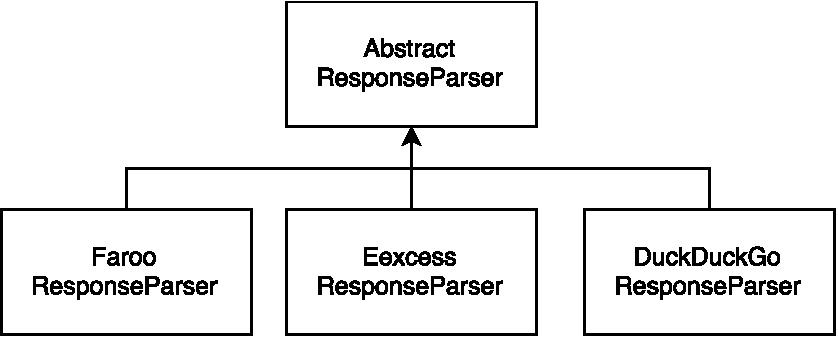
\includegraphics[]{response_parser}
		\caption{Aufbau des Moduls ResponseParse}
		\label{fig:Aufbau des Moduls ResponseParse}
\end{figure}
Der \lstinline|ResponeParser| ist für das Parsen der Antworten der Suchmaschinen in ein allgemeines Format.
Dabei wird in der aktuellen Version zwischen drei Parsern unterschieden.
\subparagraph{FarooResponseParser}
Hier werden die Antworten von Faroo verarbeitet.
\subparagraph{DuckDuckGoResponseParser}
Hier werden die Antworten von DuckDuckGO verarbeitet.
\subparagraph{EexcessResponseParser}
Hier werden die Antworten von Eexcess verarbeitet.
\subparagraph{AbstractResponseParser}
Der \lstinline|AbstractResponseParser| spezifiziert wie die untergeordneten \lstinline|ResponeParser| implementiert werden.

%\paragraph{Paragraph}
%\subparagraph{Unterparagraph}
